%%%%%%%%%%%%%%%%%%%%%%%%%%%%%%%%%%%%%%%%%%%%%%%%%%%%%%%%%%%
\section{Shape  Control using Rigid Boundaries}
\label{sec:covControl}
%%%%%%%%%%%%%%%%%%%%%%%%%%%%%%%%%%%%%%%%%%%%%%%%%%%%%%%%%%%
\begin{figure*}[!htb]
\begin{center}
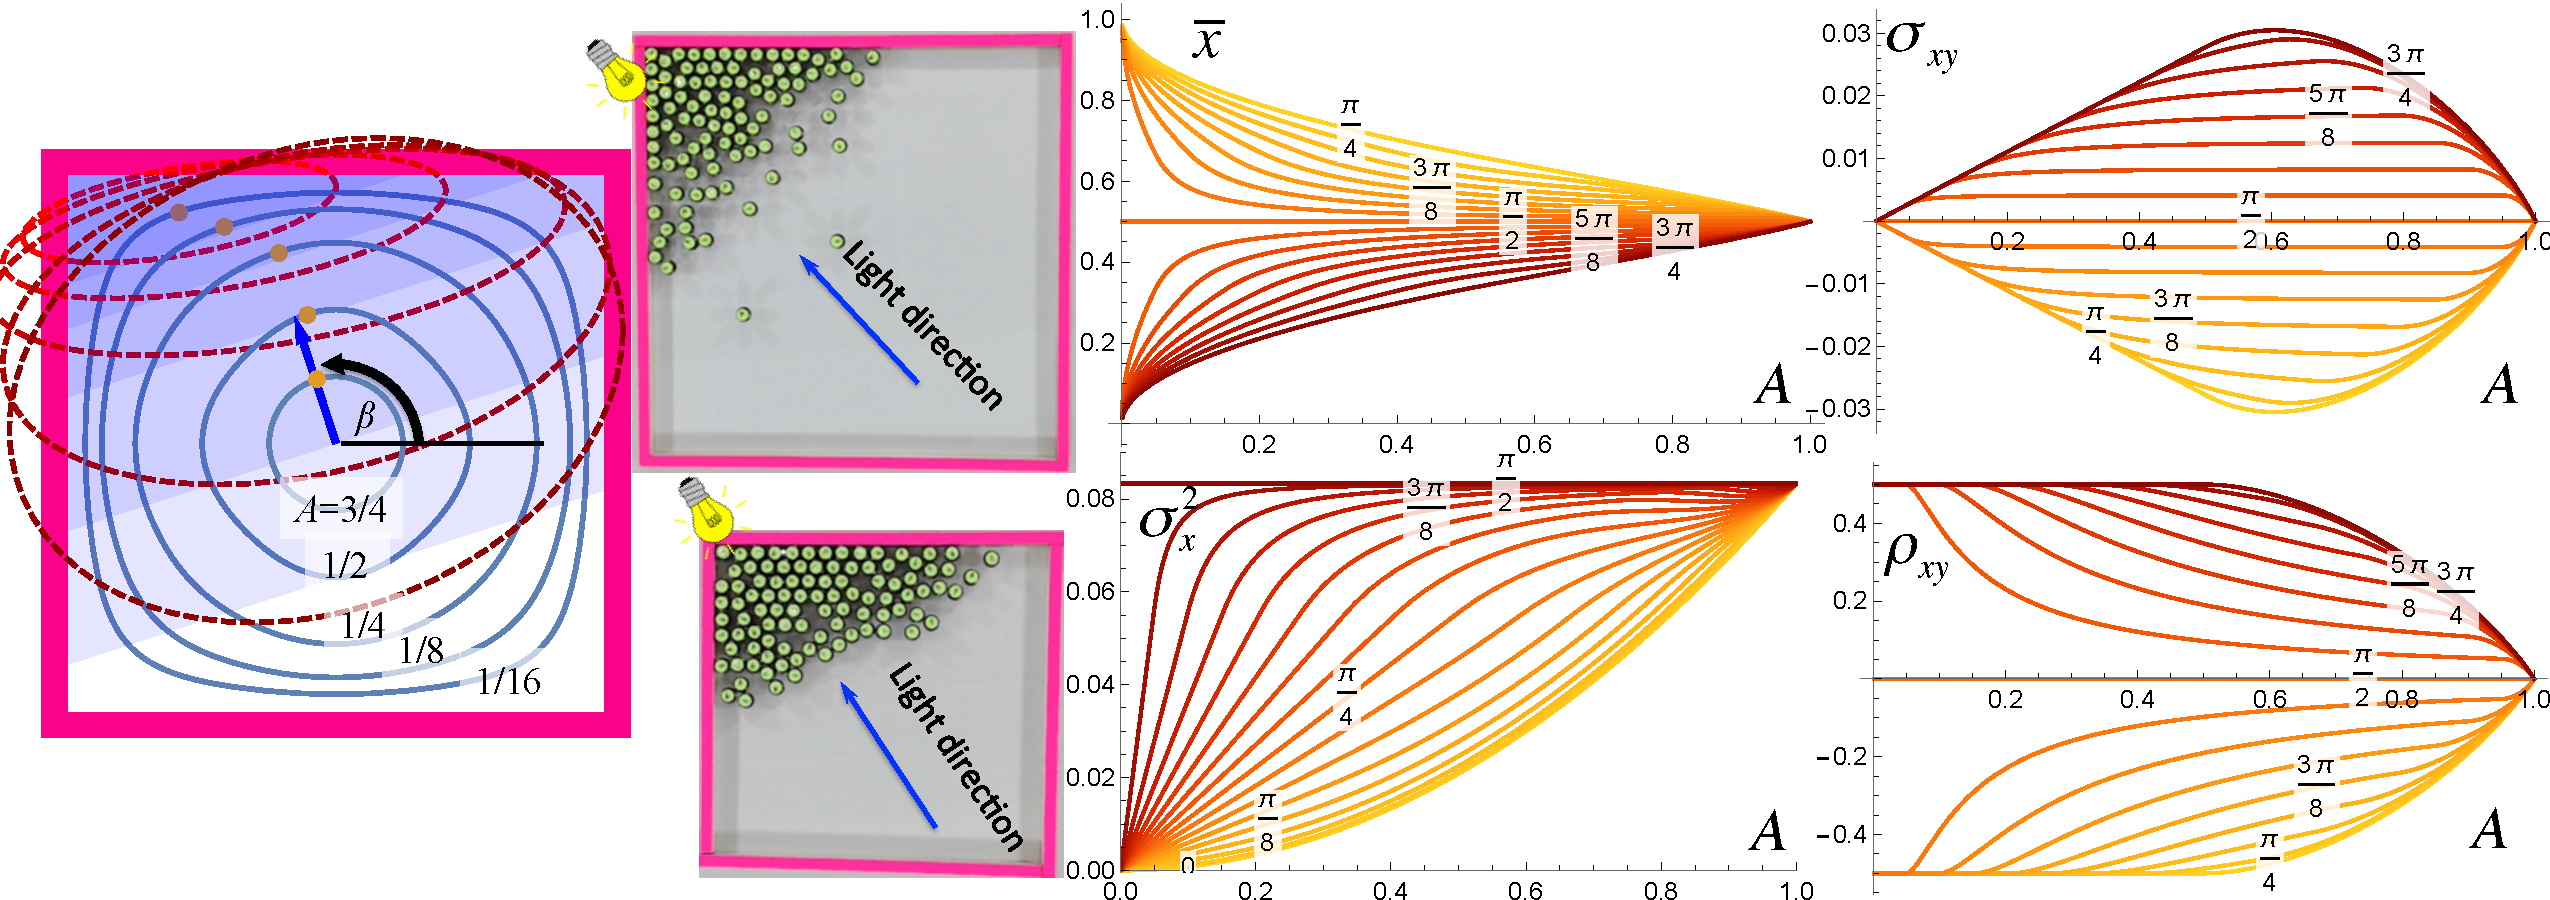
\includegraphics[width=\linewidth]{SquareFill.pdf} 
\vspace{-1em}
\caption{Pushing the swarm against a square boundary wall allows limited control of the shape of the swarm, as a function of swarm area $A$ and the commanded movement direction $\beta$. Left plot shows locus of possible mean positions for five values of $A$.  %The locus morphs from a square to a circle as $A$ increases.  The covariance ellipse for each $A$ is shown with a dashed line.
 Center shows two corresponding arrangements of kilobots.  At right is $\bar{x}(A), \sigma_{xy}(A), \sigma_x^2(A),$ and $\rho_{xy}(A)$ for a range of $\beta$ values. See online interactive demonstration at \cite{Haoran2016SwarminSquare}.
 }
\label{fig:SquareFill}
\end{center}
\end{figure*} 
\begin{figure*}[!htb]
\begin{center}
\vspace{-1em}
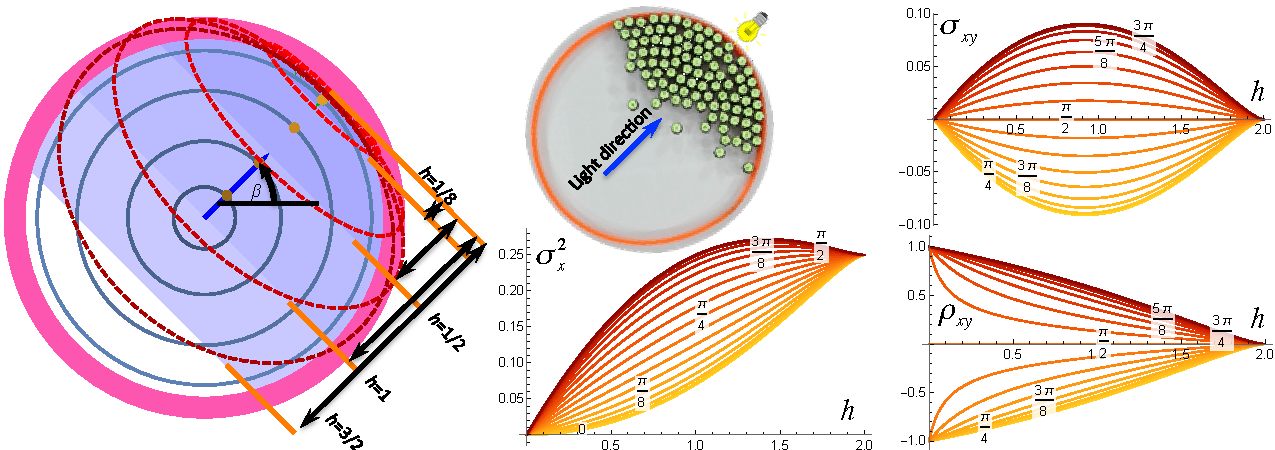
\includegraphics[width=\linewidth]{CircleFill.pdf} 
\vspace{-1em}
\caption{Pushing the swarm against a circular boundary wall allows limited control of the shape of the swarm, as a function of the fill level $h$ and the commanded movement direction $\beta$. Left plot shows locus of possible mean positions for four values of $h$. The locus of possible mean positions are concentric circles. 
At right is $\sigma_{xy}(h), \sigma_x^2(h),$ and $\rho_{xy}(h)$ for a range of $\beta$ values.
See online interactive demonstration at \cite{Haoran2016SwarminCircle}.
}  
\label{fig:CircleFill}
\end{center}
\vspace{-1em}
\end{figure*} 
Shape control using angle of repose only considers the particles that pile up on the object, but most of the particles pass by.
 This section instead focuses on shape control of the entire group when all the particles are pushed against rigid boundaries, starting by examining analytically all possible configurations in two canonical configuration spaces, and then examining the effect of boundary layer friction.

\subsection{Using boundaries: stable configurations of a swarm}\label{subsec:FluidInTank}
One method to control a swarm's shape in a bounded workspace is to simply push in a given direction until the swarm conforms to the boundary. Like fluid settling in a tank, the stable final configuration minimizes potential energy by forming a configuration with a level surface perpendicular to the push direction. The set of final configurations are parametrized by a single degree of freedom, the global input angle $\beta$.
\paragraph{Square workspace}
%The formulas for means $(\bar{x},\bar{y})$, covariance $(\sigma^2_x,\sigma^2_y,\sigma_{xy})$, and correlation $\rho_{xy}$ are as follows: 
We first examine the mean $(\bar{x},\bar{y})$, covariance $(\sigma^2_x,\sigma^2_y,\sigma_{xy})$, and correlation $\rho_{xy}$ of a large swarm of particles as they move inside a square workspace under the influence of a force pulling in the direction $\beta$. The swarm is large, but the particles are small in comparison, and together occupy a constant area $A$, $A\in [0,1]$. Under a global input, the swarm moves to a side of the workspace and forms a polygonal shape that minimizes potential energy, as shown in Fig.~\ref{fig:SquareFill}. % see also \cite{Zhao2016mathematicaSquare}.

The range for the global input angle $\beta $ is [0,2$\pi $). In this range, the swarm assumes eight different polygonal shapes. 
These shapes alternate between triangles and trapezoids when the area $A$$<$1/2, and between squares with one corner removed and trapezoids when $A$$>$1/2.


The region of integration $R$ is the polygon containing the swarm. For example, if $A<1/2$ and the force angle is $\beta$, the mean when $R$ is a triangular region in the lower-left corner is:
\begin{align}\label{eq:meanInSquareWorkspaceLL}
\bar{x}(A,\beta) &= \frac{\int_0^{\sqrt{2 A \tan (\beta)}} \left(\int_0^{\cot (\beta) \left(\sqrt{2 A \tan (\beta)}-x\right)} \, dy\right) x \, dx}{A} \nonumber \\
	&=\frac{ \sqrt{2}}{3} \sqrt{A \tan (\beta )},\\
\bar{y}(A,\beta) &= \frac{\int_0^{\sqrt{2 A \tan (\beta)}} \left(\int_0^{\cot (\beta) \left(\sqrt{2 A \tan (\beta)}-x\right)} y \, dy\right) \, dx}{A} \nonumber\\
	&=\frac{\sqrt{2}}{3}  \sqrt{A \cot (\beta )}.
\end{align}
The set of configurations are summarized in Fig.~\ref{fig:SquareFill}. For the full equations and demonstration code, see~\cite{Haoran2016SwarminSquare}. A few highlights are that the correlation is maximized $\pm$1/2 when the swarm is in a triangular shape. The covariance of a triangle is always $\pm(A/18)$. Variance is minimized in the direction of $\beta$ and maximized orthogonal to $\beta$ when the swarm is in a rectangular shape. The range of mean positions are maximized when $A$ is small.

%%%%%%%%%%%%%%%%%%%%%%%%%%%%%%%
\paragraph{Circular workspace}
Though rectangular boundaries are common in artificial workspaces, biological workspaces are usually rounded.
Similar calculations can be made for a circular workspace.  The workspace is a circle centered at (0,0) with radius 1 and thus area $\pi$.
For notational simplicity, the swarm is parameterized by the global control input signal $\beta$ and the fill-level $h\in[0,2]$.  
Under a global input, the particle swarm fills the region under a chord with area
\begin{align}
A(h) = \arccos(1-h)-(1-h) \sqrt{(2-h) h}.
\end{align}
For a circular workspace, the locus of mean positions are aligned with $\beta$ and the mean position is at radius $r(h)$ from the center which is
\begin{align}
r(h) = \frac{2 (-(h-2) h)^{3/2}}{3 \left(\sqrt{-(h-2) h} (h-1)+\arccos(1-h)\right)}.
\end{align}
Variance $\sigma^2_x(\beta,h)$ is maximized at $\beta = \pi/2+n \pi$ and $h\approx1.43$, while covariance is maximized at $\beta = \pi3/4+n \pi$ and $h\approx0.92.$ For small $h$ values, correlation approaches $\pm1$. Results are displayed in Fig.~\ref{fig:CircleFill}.  For the full equations and demonstration code, see~\cite{Haoran2016SwarminCircle}.%, see also \cite{Zhao2016mathematica}.

%Smashing the swarm to the corner walls will cause some correlation between \emph{x} and \emph{y} axes. Eq. ~\ref{eq:Wall} shows the relation between number of particles and area provided and the correlation we can reach with it.
%%TODO: ADD the equation for showing the correlation Vs area, vs number of particles
% This equation shows that we are not able to reach high correlations bigger than $|0.5|$. Fig. ~\ref{fig:wallCorrelation} shows the different mean positions and correlations we are able to reach. There are ways and corridors that the swarm needs to pass and also to keep the majority of it. If we use the wall corners technique and the way needs a very high correlation to pass, a remarkable number of the swarm members will be lost, and we may lose track of them due to their small size. Meanwhile, the variance of the swarm would get bigger and bigger that it would not anymore be able to deliver sufficient payloads. For this reason we have thought another idea which uses \emph{friction} to make correlations.
%


\subsection{Using boundaries: friction and boundary layers}\label{subsec:WallFriction}
Global inputs move a swarm uniformly.  
Shape control requires breaking this uniform symmetry.  
A swarm inside an axis-aligned rectangular workspace can reduce variance normal to a wall by simply pushing the swarm into the boundary. 
If the swarm can flow around each other, pushing the swarm into a boundary produces the limited set of configurations presented in Sec.~\ref{subsec:FluidInTank}.
%Controlling covariance by pushing the swarm into a boundary requires changes to the boundary.  
%An obstacle in the lower-right corner is enough to generate positive covariance, but generating both positive and negative covariance requires additional obstacles.  
%Requiring a special obstacle configuration also makes shape control dependent on the local environment. 
Instead of pushing our particles directly into a wall, the following sections examine an oblique approach  using boundaries that generate friction with the particles. 
 These frictional forces are  sufficient to break the symmetry caused by uniform inputs.  
 Particles touching a wall have a friction force that opposes movement along the boundary.  
This causes particles along the boundary to move more slowly than particles in free-space. 
  
Let the control input be a vector force $\vec{F}$ with magnitude $F$ and orientation $\theta$ with respect to a line perpendicular to and into the nearest boundary. $N$ is the normal or perpendicular force between the particle and the boundary. The force of friction $F_f$ is nonzero if the particle is in contact with the boundary and  $\sin(\theta) < 0$. The resulting net force on the particle, $F_{\text{\emph{forward}}}$, is aligned with the wall and given by
\begin{align}
F_{\text{\emph{forward}}} &=  F \sin(\theta) - F_f , \nonumber \\
\text{where }  F_f &= \begin{cases}  \mu_f N, &  \mu_f N < F \sin(\theta)  \label{eq:frictionmodel}  \\
F \sin(\theta), & \text{else} \end{cases} \\ %\sign(F \sin(\theta) ) \cdot  \max(0, | F sin\theta |- |F_f|)
\text{and } N &= F \cos(\theta) .\nonumber
\end{align}
 Fig.~\ref{fig:friction} shows the resultant forces on two particles when one is touching a wall. 
Though each receives the same inputs,  they experience different net forces.
  For ease of analysis, the following algorithms assume $\mu_f$ is infinite and particles touching the wall are prevented from sliding along the wall.
This means that if one particle is touching the wall and another particle is free, the touching particle will not move when the control input is parallel or into the wall. 
There are many alternate models of friction that also break control symmetry. Fig.~\ref{fig:friction}c shows fluid flow along a boundary.  Fluid in the free-flow region moves uniformly, but flow decreases to zero in the boundary layer \cite{fluidMechanics}.  Force in such a system can be calculated as
\begin{align}
%u(y) = u_0 \left(1- \frac{(y-h)^2}{h^2}\right) = u_0 \frac{y}{h} \left(2- \frac{y}{h}\right) \label{eq:boundarylayerflow} THiS EQUATION IS TERRIBLE! PLOT IT.
F_{\text{\emph{forward}}}(y) &= F - F_f\begin{cases}  \frac{h-y}{h}   , &  y<h \label{eq:boundarylayerflow} \\
0, & \text{else} \end{cases}.
\end{align}

\begin{figure}[h]
\begin{center}
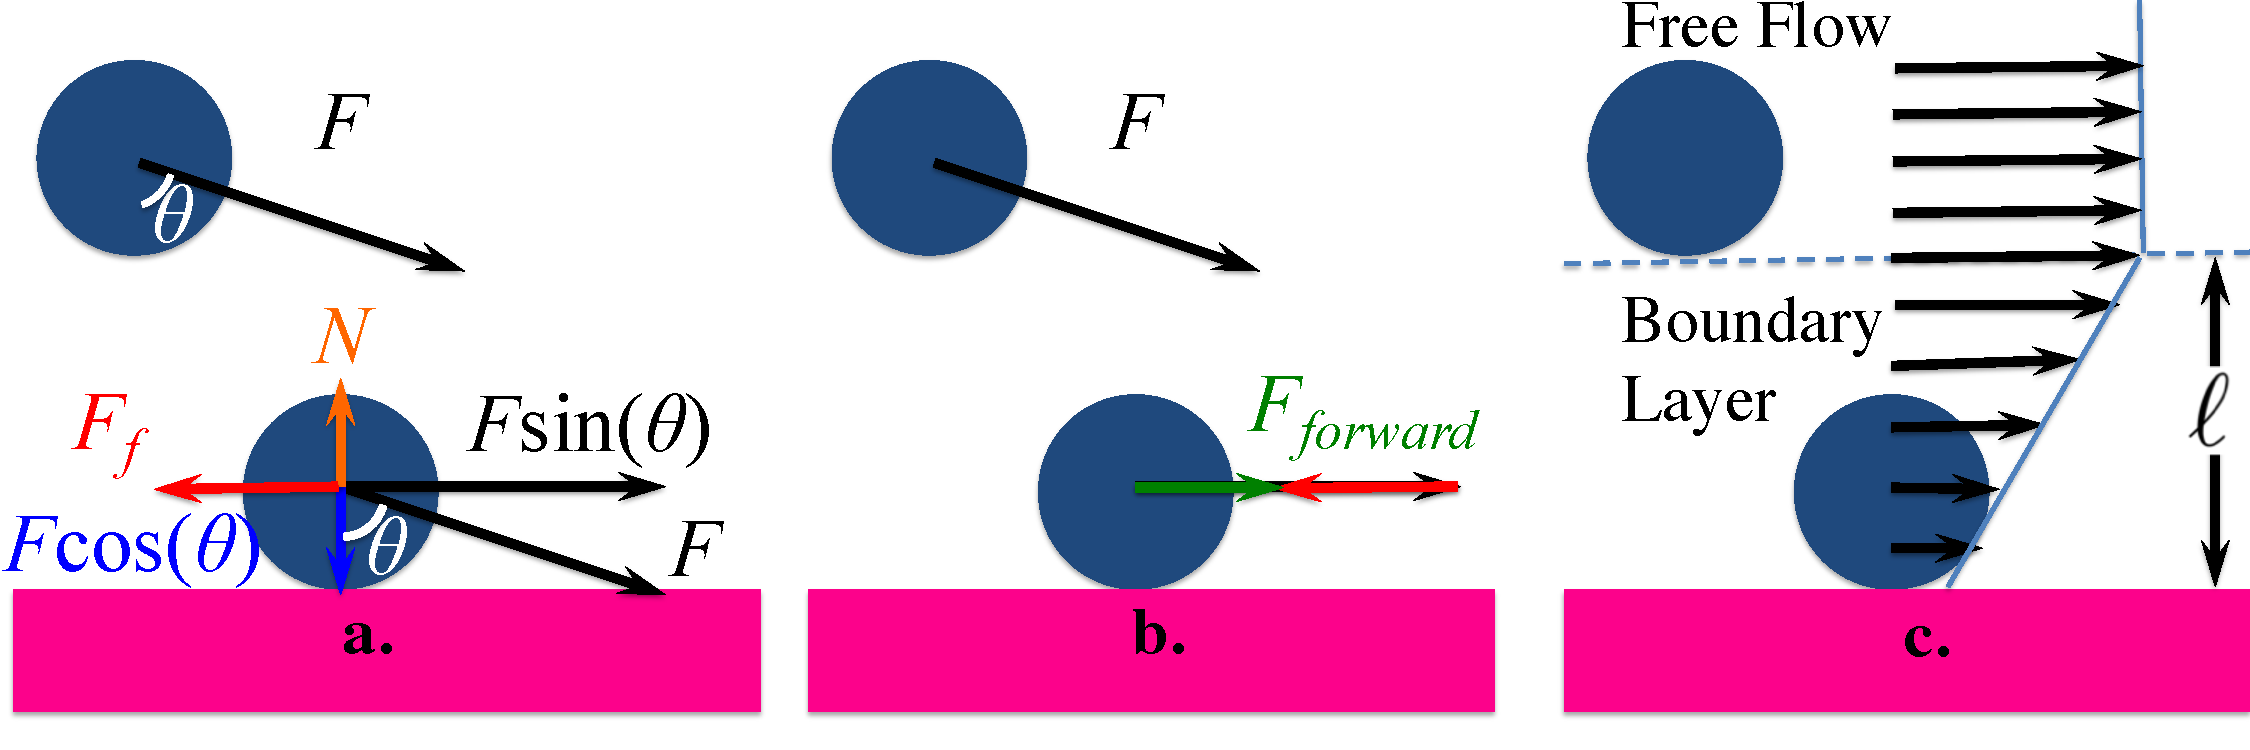
\includegraphics[width=0.8\columnwidth]{friction.pdf} 
\vspace{-1em}
\caption{(a,b) Wall friction reduces the force for going forward $F_{\text{\emph{forward}}}$ on a particle near a wall, but not for a free particle. (c) velocity of a fluid reduces to zero at the boundary.
\label{fig:friction}
}\vspace{-1em}
\end{center}
\end{figure} 




\subsection{Maximizing correlation using wall friction}\label{subsec:ClosedLoopCovarianceControl}
%Using the environment to individually move $n$ particles to goal positions in Alg. \ref{alg:PosControlNRobots} requires $O(n^2)$ time, while  Alg. \ref{alg:optimalAlg} can only control two particles. The controllers in Section \ref{sec:theory} are efficient because they require only a single move but the range of possible configurations are limited. This section presents an efficient technique to generate desired correlations.

Assume an obstacle-free, bounded, unit-size, square workspace. 
 As shown in Fig.~\ref{fig:SquareFill}, the maximum correlation occurs when the swarm is pushed in the direction $\beta = 3\pi/4$. 
 This correlation as a function of swarm area $A$ is never larger than 1/2, and the maximum correlation decays to 0 as $A$ grows to 1. By  \eqref{eq:covAndcorrInSquareWorkspace}, this maximum correlation is
\begin{align} \label{eq:GravityCorrelation}
\rho_{xy} =  \begin{cases}  \frac{1}{2}  , &  0\le A\le \frac{1}{2}  \\
% \frac{3 A (2 (A-2) A+1)}{4 A \left(A^2+3 \sqrt{2-2 A}-6\right)-12 \sqrt{2-2 A}+17}-1
 \frac{3 A (2 (A-2) A+1)}{4 A^3-24 A+\sqrt{2} (12 A-12) \sqrt{1-A}+17}-1
 , & \frac{1}{2} \le A\le 1
\end{cases}.
\end{align}
 If friction obeys the linear boundary layer model of \eqref{eq:boundarylayerflow} with boundary layer thickness $h$ and maximum friction $F_f$ equal to the maximum applied force $F$, we can generate  larger correlations.
 If the swarm size is smaller than $A \approx 0.43$ and the boundary layer is sufficiently thick we can generate correlations larger than 1/2  using boundary friction.

 Assume that the swarm is initialized in the lower-left corner, in a rectangle of width $w$ and height $A/w$. 
 Such a rectangular configuration can be accomplished using the variance controllers from \cite{ShahrokhiIROS2015}. 
  If the swarm is then commanded to move a distance $L$ to the right, components of the swarm outside the boundary friction layer of height $h$ move further than components near the boundary. 
   The swarm is contained in a region $R$ composed of no more than three stacked components: at bottom a parallelogram inclined to the right top, at middle a rectangle, and at top a parallelogram inclined to the left top. These regions can be defined by the rectangle's left side, bottom, and top (see Fig.~\ref{fig:ControlledCorrelation}):
\begin{align}
r_{\text{left}} &= \min \left(L,1-w \right),\nonumber \\
r_{\text{bottom}} &=\min \left(\frac{A}{w}, h\frac{r_{\textrm{left}}}{L}  \right) \text{and}\nonumber \\
r_{\text{top}}  &= \min \left(\frac{A}{w}, 1-h\frac{r_{\text{left}}}{L}  \right).
\end{align}
If $\frac{A}{w} \le r_{\text{top}}$ the top parallelogram has no area. 
 Similarly, if $r_{\text{top}} \le r_{\text{bottom}}$ the rectangle has no area. 
The mean, variance, and correlation are calculated  using \eqref{eq:meanInSquareWorkspace}, \eqref{eq:varInSquareWorkspace}, and \eqref{eq:covAndcorrInSquareWorkspace} over the region $R$:
\begin{align} \iint_R f(x,y) \, dx \,dy &=  \int_0^{r_{\text{bottom}}}  \int_{\frac{L}{h}y}^{\frac{L}{h}y+w}  f(x,y)  dx \, dy \label{eq:correlationFriction} \\
&+\int_{r_{\text{bottom}}}^{r_{\text{top}}} \int_{r_{\text{left}}}^{r_{\text{left}} +w} f(x,y)    dx \, dy \nonumber\\
&+\int_{r_{\text{top}}}^{\frac{A}{w}} \int_{-\frac{L (y-r_{\text{top}})}{h}+r_{\text{left}}}^{r_{\text{left}}+w-\frac{L (y-r_{\text{top}})}{h}} f(x,y)   dx \, dy .\nonumber
\end{align}
 
 Given an environment parameterized by $A$ and $h$, efficient correlation control consists of choosing the $w,L$ pair  that generates the desired positive correlation.
  Negative correlations can be generated by initializing the swarm in the upper left, or lower right.

\subsection{Efficient control of correlation}
\begin{figure}
\begin{center}
	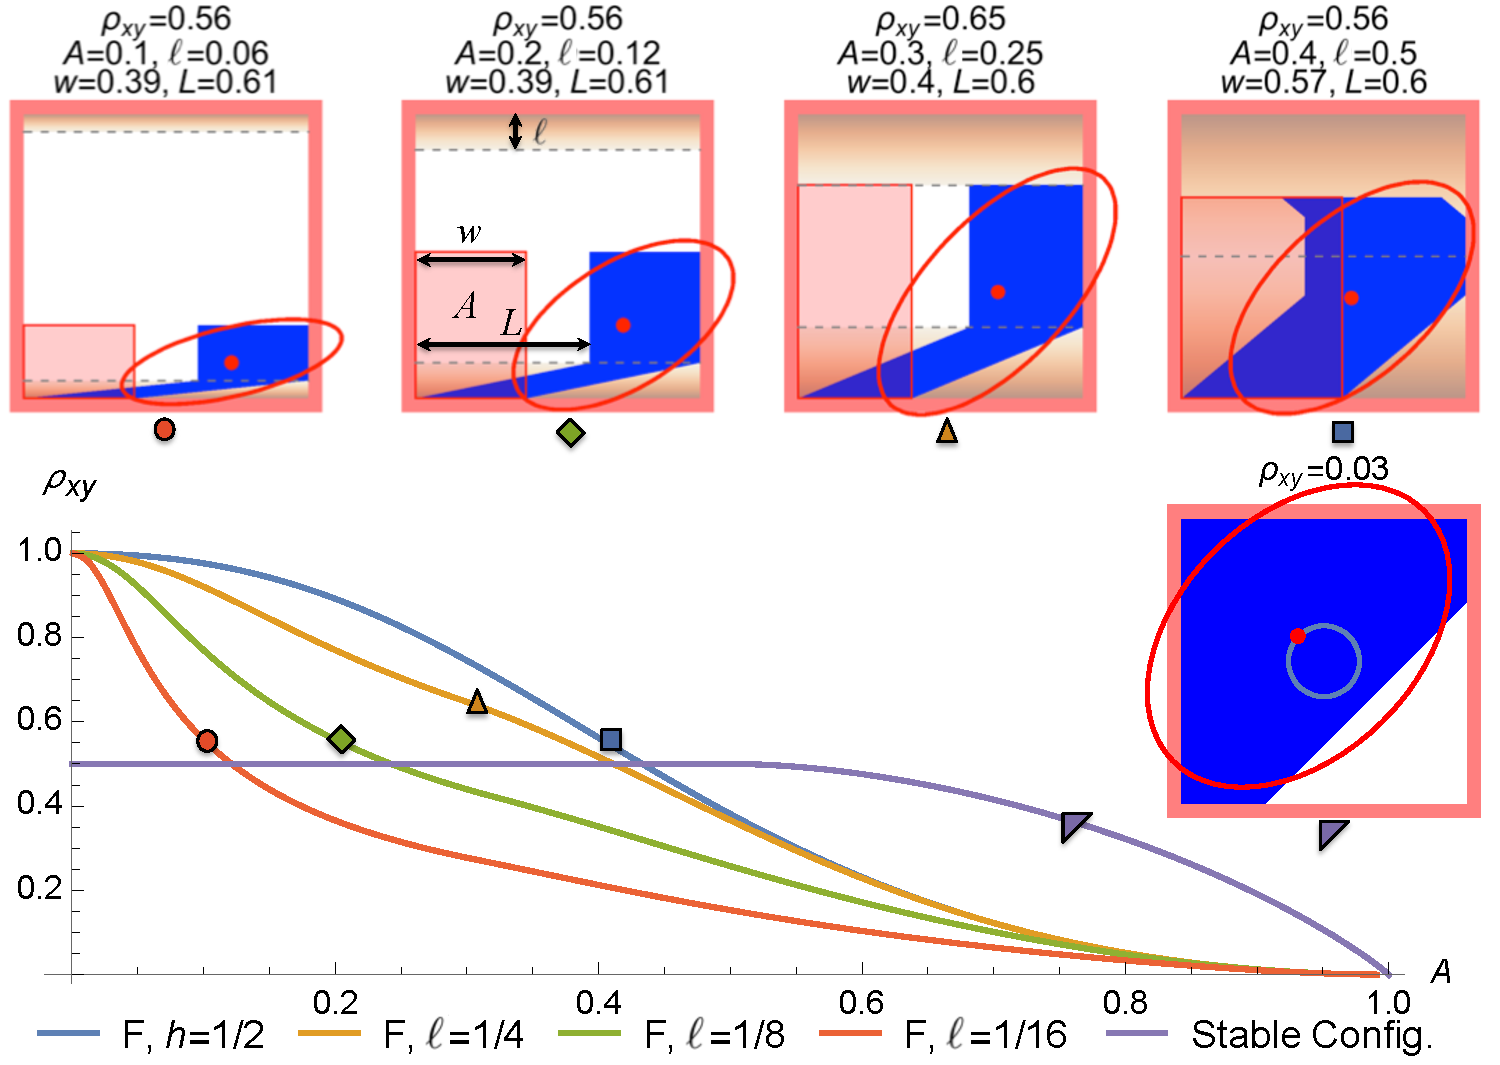
\includegraphics[width=\columnwidth]{ControlledCorrelation.pdf}
\end{center}
\vspace{-1em}
\caption{\label{fig:ControlledCorrelation}
Analytical results comparing maximum correlation $\rho_{xy}$. Lines labeled \textsf{F} use the boundary layer friction model of \eqref{eq:correlationFriction} with four boundary layer thicknesses $h$ and the stable triangular configuration \eqref{eq:GravityCorrelation}.
}\end{figure}

%A set of simulations were conducted to demonstrate the importance of boundary friction.  
This section examines maximum correlation values as a function of  $w,L$ using \eqref{eq:correlationFriction}
from Section  \ref{subsec:ClosedLoopCovarianceControl}. 
The maximum correlation using boundary layer friction $\displaystyle  \max_{w,L} \left( \rho(A,h,w,L) \right)$ can be found by gradient descent, as shown in Fig.~\ref{fig:ControlledCorrelation}. 
For swarms with small area, this method enables generating the full range of correlations $\pm 1$. %, while the stable configuration method from Section \ref{sec:theory} could only generate correlations $\pm 1/2$.  
  As  the swarm area $A$ increases above $\approx 0.43$, the stable configuration method is more effective.
Larger boundary layers $h$ enable more control of correlation.
%  The video attachment shows efficient control of correlation with simulations using the 2D physics engine Box2D~\cite{catto2010box2d} and 144 disc-shaped robots with boundary layer model \eqref{eq:boundarylayerflow}.





\section{Experiments}\label{sec:Experiments}
This section reviews three demonstrations of efficient shape control of many particles.
\subsection{Hardware experiment: particle angle of repose}
In this section we varied the approach angle to shape a swarm with a characteristic angle of repose.  
We then showed how the angle of repose can be increased by decreasing the magnitude of the force that moves the particles.
%
\begin{figure}
\begin{center}
	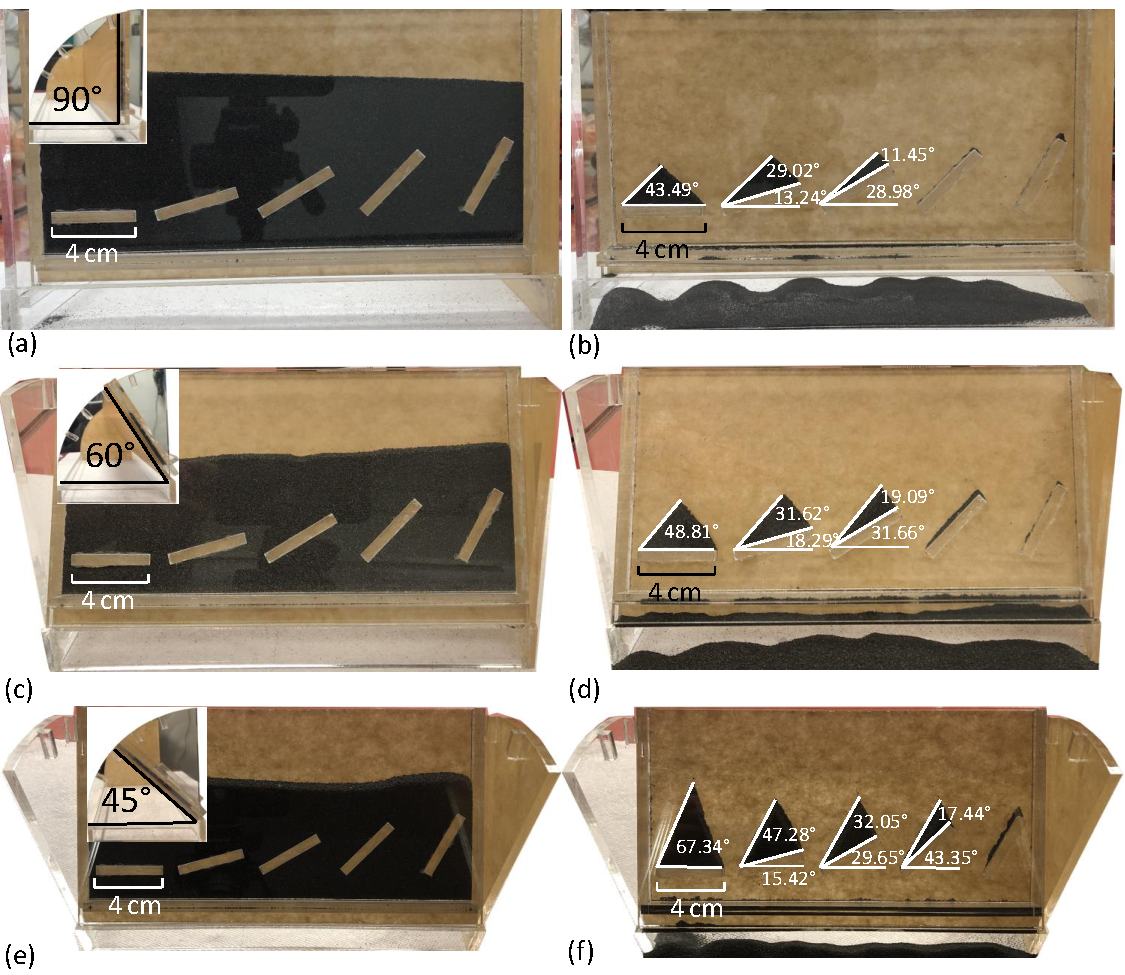
\includegraphics[width=\columnwidth]{aorPlot.pdf}
\end{center}
\caption{\label{fig:angleOfReposeExp}
Experimental data using iron particles, varying angle of attack, and three tilt angles to vary the force applied by gravity.
}
\end{figure}
%
%\begin{figure}
%\begin{center}
%	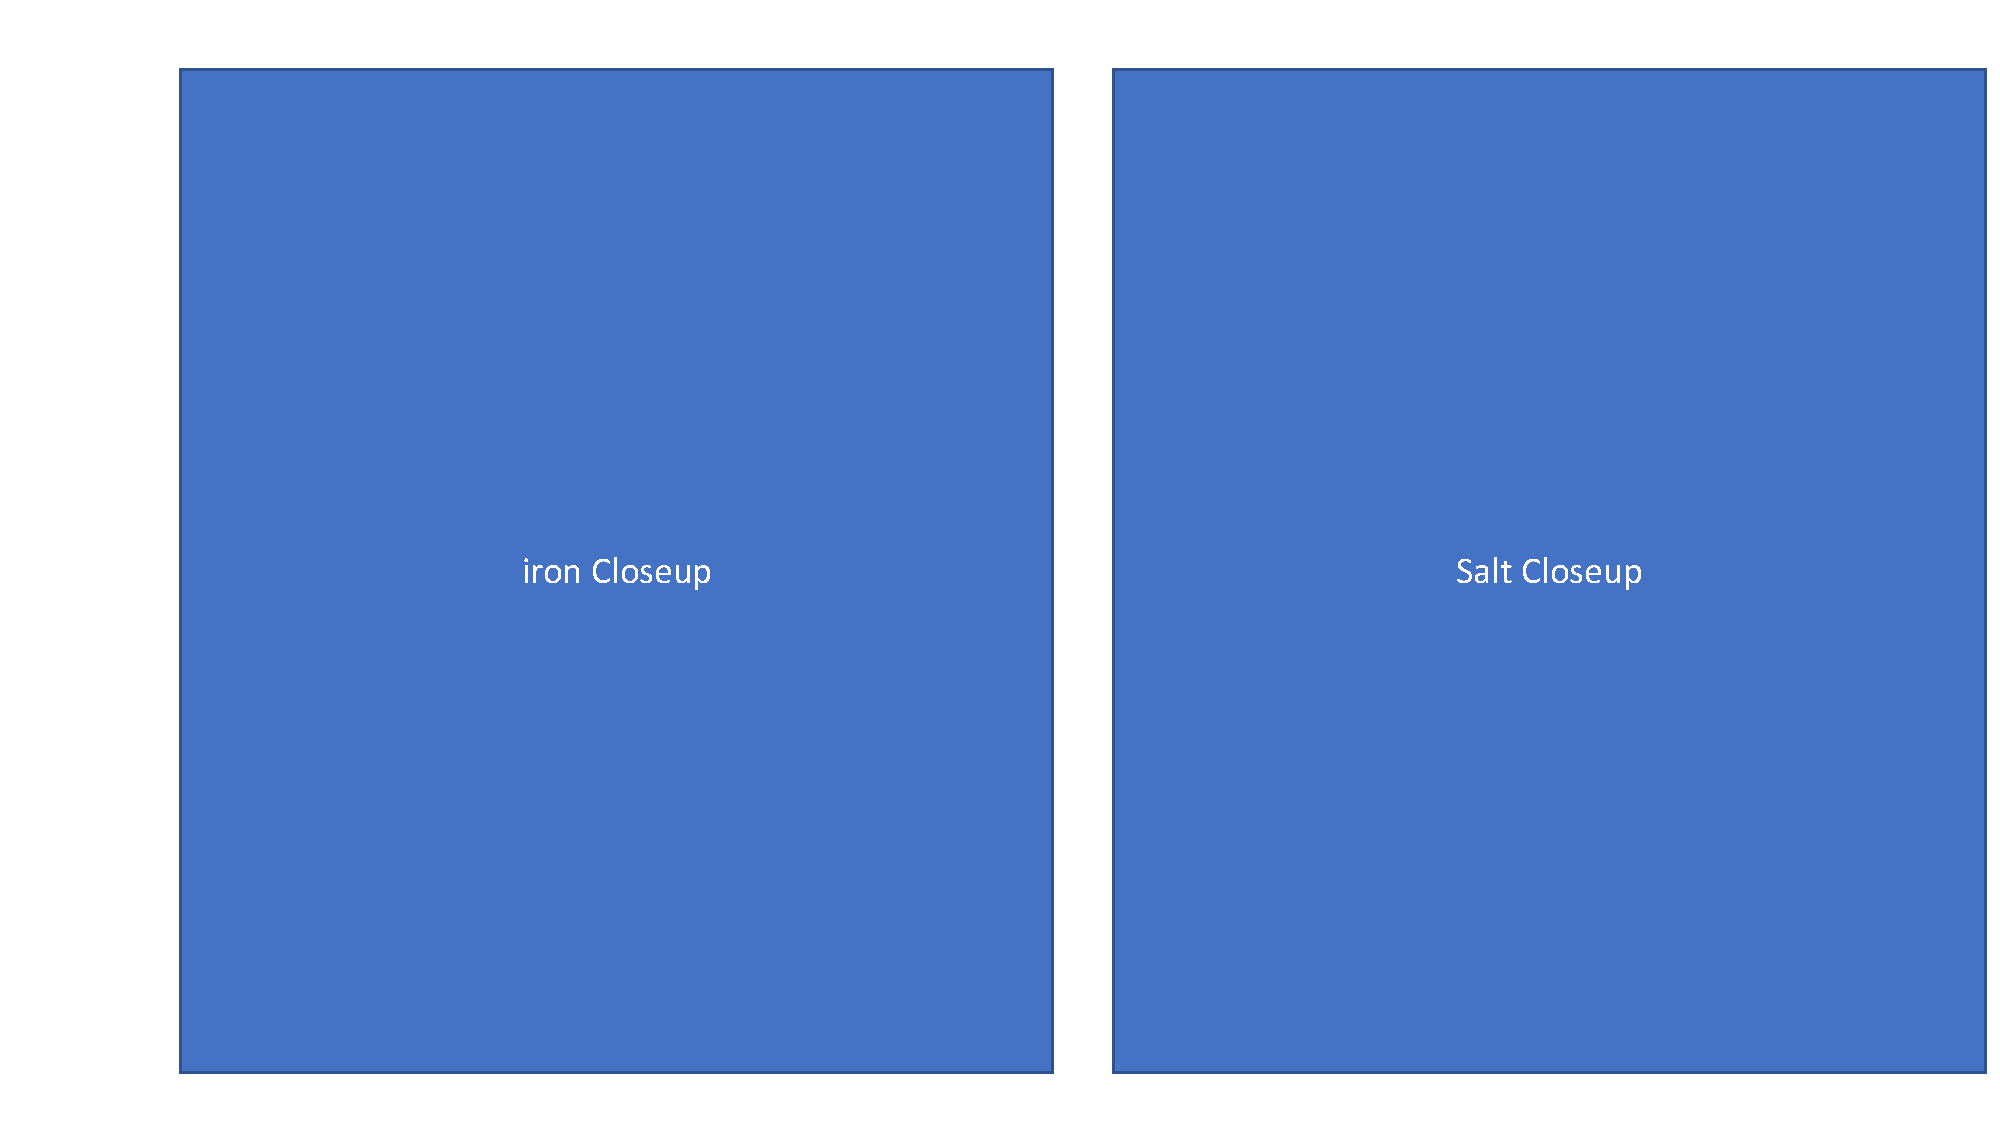
\includegraphics[width=\columnwidth]{ironAndSaltCloseup.pdf}
%\end{center}
%\caption{\label{fig:ironAndSaltCloseup}
%Magnified image of salt and iron at angle of repose.
%}
%\end{figure}
%
The particles used are iron filings (?Company name and particle size?), and the motive force is gravity. 
The particles were poured into a frame composed of two sheets of acrylic with ?? mm spacing between. Five 40 mm rods were epoxied between the sheets at angles 
 $\{0^\circ,15^\circ, 30^\circ, 45^\circ, 60^\circ \}$, generating angle of attacks $\beta = \{90^\circ,75^\circ, 60^\circ, 45^\circ, 30^\circ \}$.
 The frame was tested at three tilt angles with respect to horizontal: $\beta = \{90^\circ,60^\circ, 45^\circ \}$, resulting in $\{100,87, 71\}\%$ of the gravitational force.
 For each test the bottom of the frame was removed to allow unsupported particles to escape and the shape of the remaining particles was measured from photographs taken by a tripod-mounted camera inclined at the same tilt angle as the frame.
  The decreasing tilt angles resulting in increasing angle of repose values: $\alpha = \{42^\circ,50^\circ, 63^\circ \}$
These experiments show how the pile of particles can be used to convey two scalar values: the force applied and the attack angle.  We can also apply varying levels of force and torque to the rod according to \eqref{eq:ForceAOR} and \eqref{eq:TorqueAOR}.

\subsection{Hardware experiment: kilobot angle of repose}
We varied the approach angle to shape a swarm of Kilobots \cite{rubenstein2014programmable} with a characteristic angle of repose. 
 A Kilobot is a three-centimeter diameter,  low-cost robot. In our experiments, these robots were programmed to go toward the brightest light in the room. The experimental setup is shown in Fig. \ref{fig:SetUp}, also showing angle of repose of the Kilobots with  the pink rod at three angles of attack: 90$^\circ$, 67.5$^\circ$ and 45$^\circ$. The green lines show the triangle shape the robots pile up into. The cyan star is the center of mass of the rod, and the mean position and variance of the robots are shown with  red stars and red ellipses.
\begin{figure}
\begin{center}
	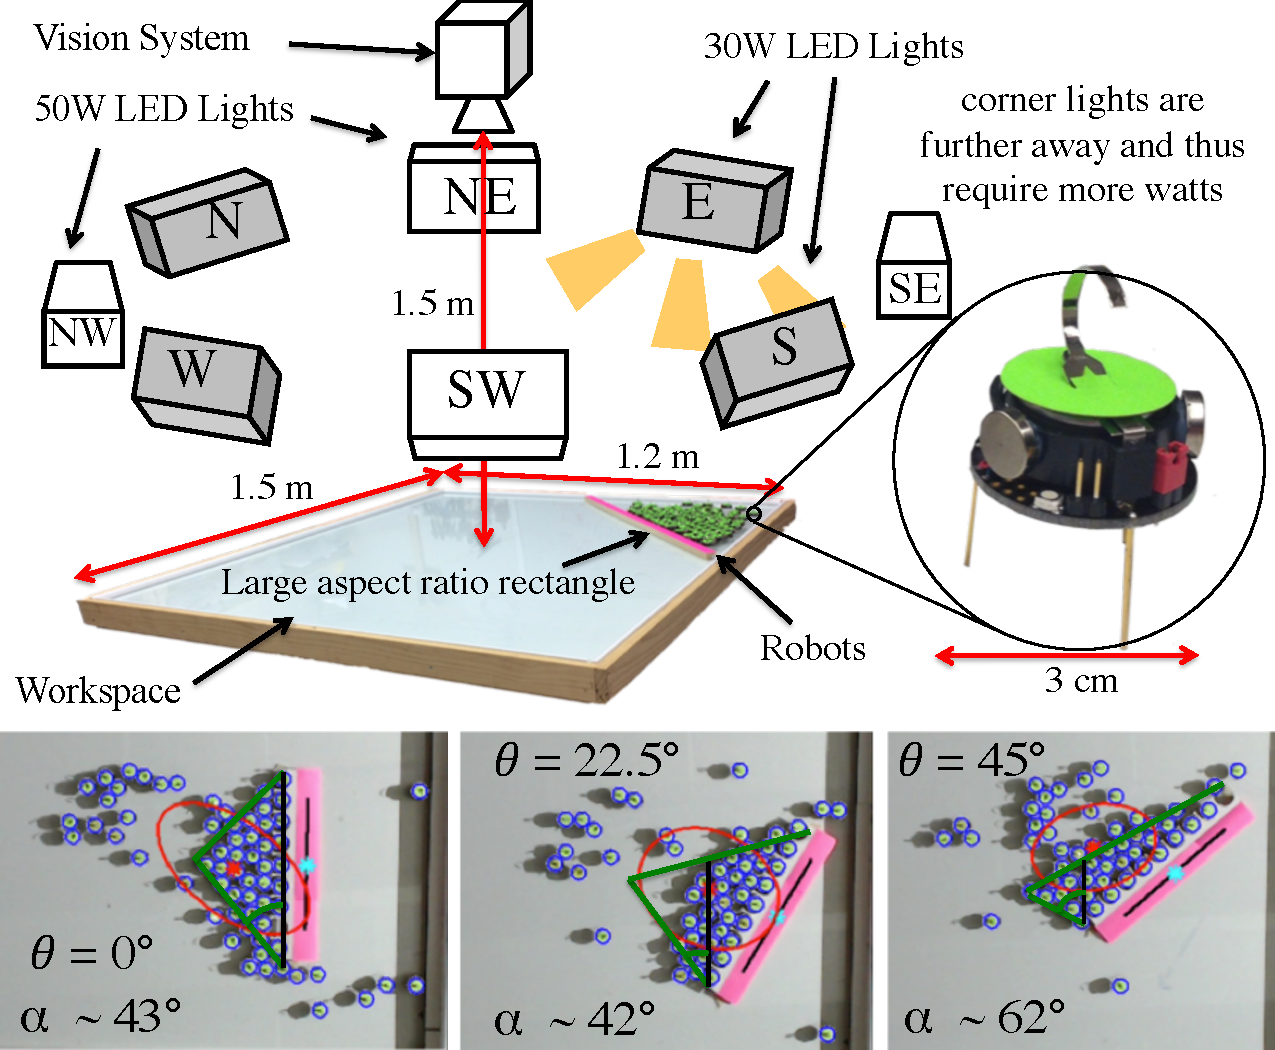
\includegraphics[width=\columnwidth]{SetUp.pdf}
\end{center}
\caption{\label{fig:SetUp}
Steering Kilobots with lights and characteristic shape formed by Kilobot angle of repose for three angle of attacks.
}
\end{figure}




%\textcolor{red}{TODO: Shiva will insert the kilobot images and a couple of sentences, and a couple of sentences about kilobots}


\subsection{Hardware experiment: control of covariance}
To demonstrate covariance control, up to 100 kilobots were placed on the workspace and manually steered with lights, using friction with the boundary walls to vary the covariance from  -4000 to 3000 cm$^2$.  The resulting covariance is plotted in Fig.~\ref{fig:covExperiment}, along with snapshots of the swarm.




\begin{figure}
\begin{center}
	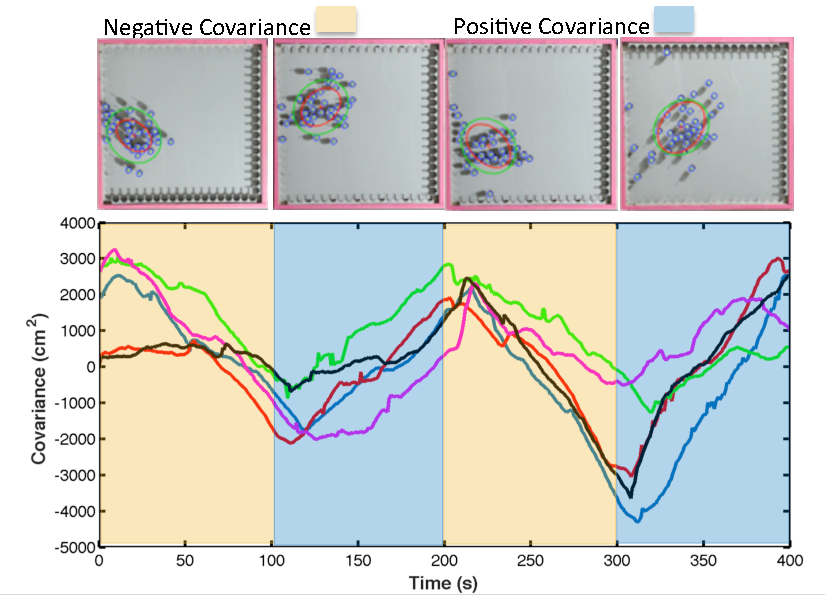
\includegraphics[width=\columnwidth]{newExperiment.pdf}
\end{center}
%\vspace{-1em}
\caption{\label{fig:covExperiment}
Hardware demonstration steering $\approx 50$ kilobot robots to desired covariance. The goal covariance is negative in first 100 seconds and is positive in the next 100 seconds. The actual covariance is shown in different trials. Frames above the plot show output from machine vision system and an overlaid covariance ellipse.
%\vspace{-2.5 em}
}
\end{figure}

